\hypertarget{obsah-kurzu}{%
\chapter{Obsah kurzu}\label{obsah-kurzu}}

V~poslední kapitole si představíme vytvořený online kurz pro výuku datové analytiky. Tuto kapitolu dělíme do několika vzájemně provázaných částí, z~nichž každá reflektuje odlišnou oblast návrhu a~implementace online kurzu.

\hypertarget{prux16fchod}{%
\section{Průchod}\label{prux16fchod}}

V~první částí se zaměříme na obecný průchod kurzem -- popíšeme, jak je kurz navržen po strukturální stránce a~jakým způsobem student prochází jednotlivými částmi\footnote{V současné chvíli probíhá redesign webových stránek firmy Digiskills, proto se mohou některé přiložené obrázky lehce vizuálně lišit od aktuální podoby kurzu.}.

Hlavní část kurzu je tvořena sedmi hlavními obsahovými bloky, z~nichž se každý zabývá jedním určitým tématem, které na sebe přímo navazují a~představují tak hrubou strukturu online kurzu (viz Obrázek \ref{digi-bloky}). Od studenta se tedy očekává lineární postup směrem od prvního do poslední obsahového bloku, nicméně je i~tak studujícímu umožněno procházet libovolný blok dle aktuálních potřeb (a~to ať už ty minulé např. z~důvodu ujasnění si již probraných témat nebo ty nenavštívené např. kvůli zjištění celkové časové náročnosti kurzu).

Mimo tyto ústřední bloky e-learning na začátku obsahuje úvodní text, jehož cílem je studenta motivovat ke studiu a~v~co největší stručnosti popsat obsah celého kurzu. Zároveň je pod touto úvodní kartou umístěn malý ukazatel progresu s~počtem splněných aktivit (viz další odstavec) spolu s~podkartou \emph{Užitečný tip}, která slouží v~rámci ekosystému kurzů Digiskills k~nasměrování na integrovaného chatbota (viz Obrázek \ref{digi-uvod}).

Základní jednotkou kurzu jsou již zmíněné aktivity, jež jsou vždy zanořeny do daného obsahového bloku (viz Obrázek \ref{digi-blok}). Těchto aktivit je v~celém kurzu v~současné chvíli 23 a~jsou do jednotlivých bloků logicky uspořádány dle následující šablony:

\begin{itemize}
\tightlist
\item
  úvodní aktivita, která představuje studentovi dané téma a~kontextualizuje jej v~rámci aktivit minulých a~následujících;
\item
  1--3 aktivity zpracovávající konkrétní část tématu;
\item
  1--2 závěrečné aktivity, jež shrnují dané téma a~pobízí studenta k~vlastní práci ať už prostřednictvím kvízů či praktických úkolů (viz Obrázek \ref{digi-aktivity}).
\end{itemize}

\begin{figure}[hb!]   
    \centering
    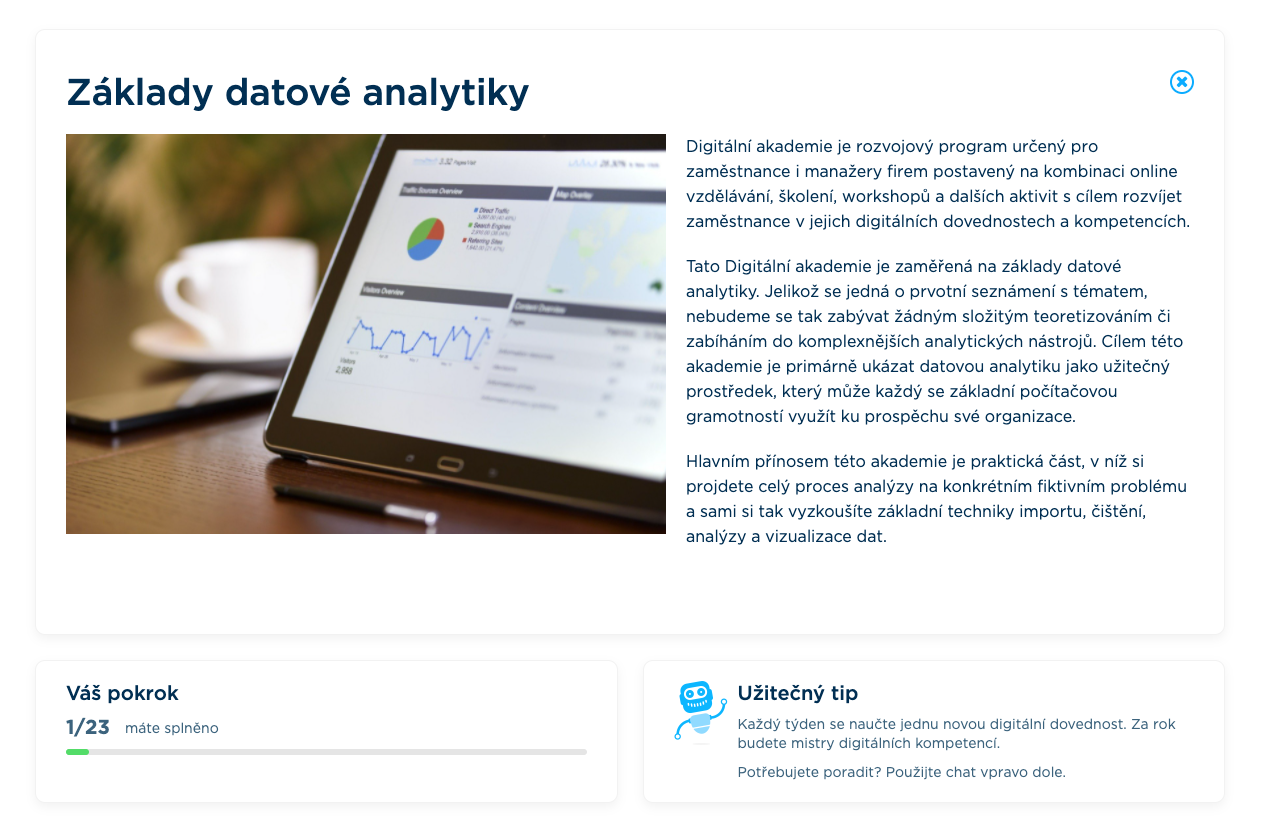
\includegraphics[width=\textwidth]{digi-uvod}  
    \caption{Úvodní obrazovka s~představením kurzu spolu s~ukazatelem progresu a~s~podkartou týkající se užitečného tipu.}
    \label{digi-uvod}
\end{figure}

\begin{figure}[hb!]   
    \centering
    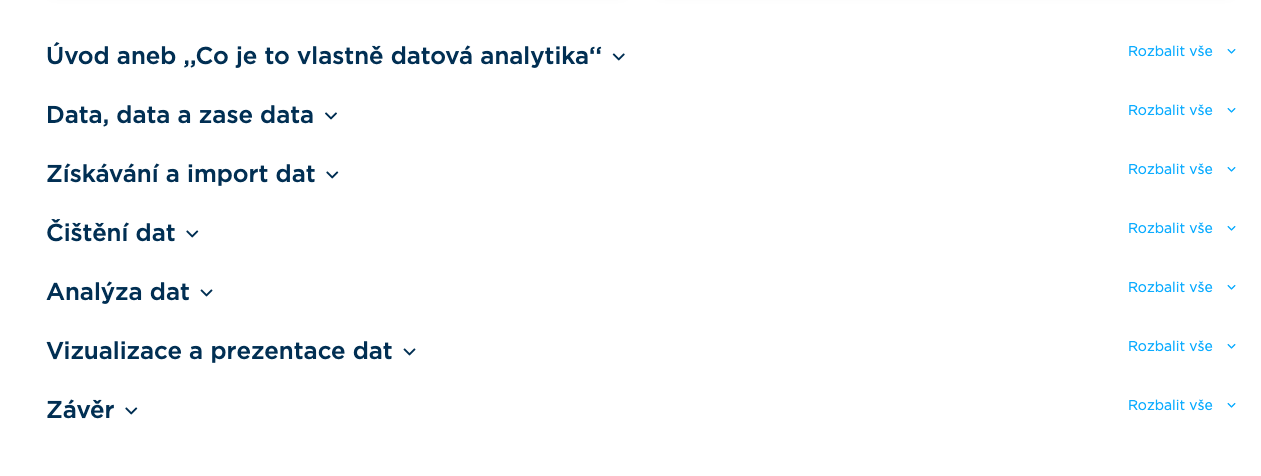
\includegraphics[width=\textwidth]{digi-bloky}  
    \caption{Nerozbalený výčet všech obsahových bloků}
    \label{digi-bloky}
\end{figure}

\begin{figure}[hb!]   
    \centering
    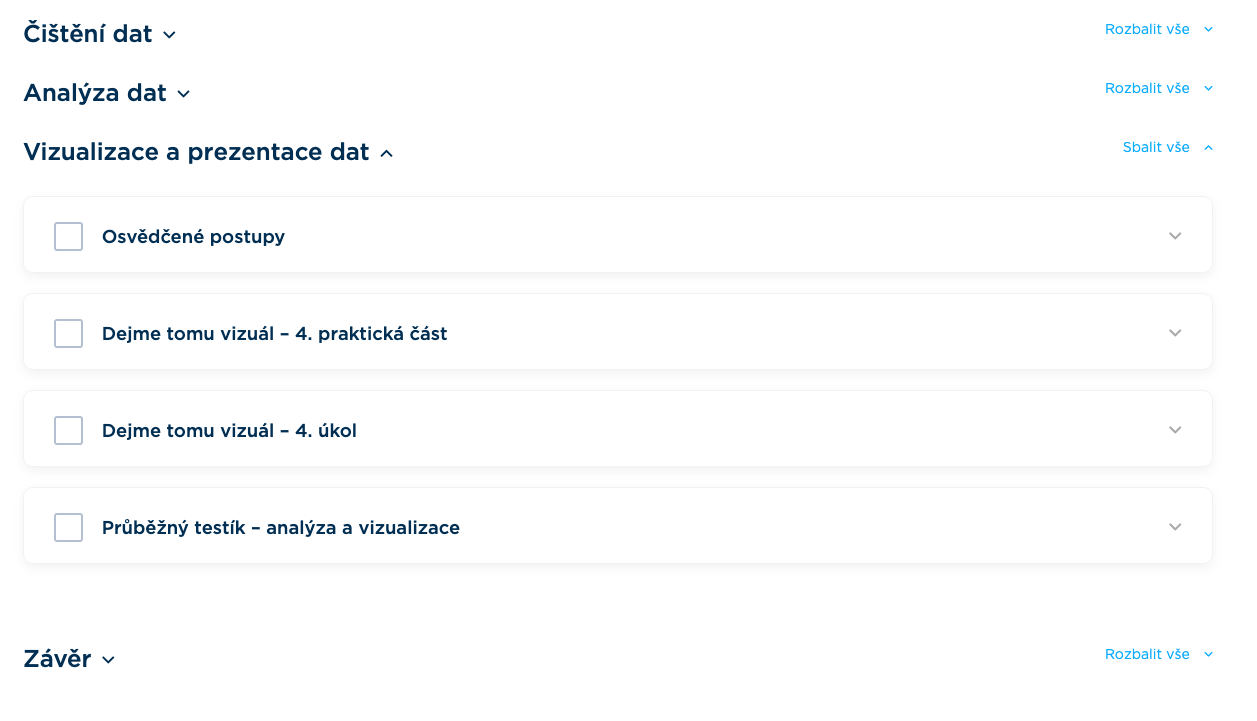
\includegraphics[width=\textwidth]{digi-blok}  
    \caption{Vnořené aktivity vztahující se ke obsahovému bloku Vizualizace a~prezentace dat}
    \label{digi-blok}
\end{figure}

\begin{figure}[hb!]   
    \centering
    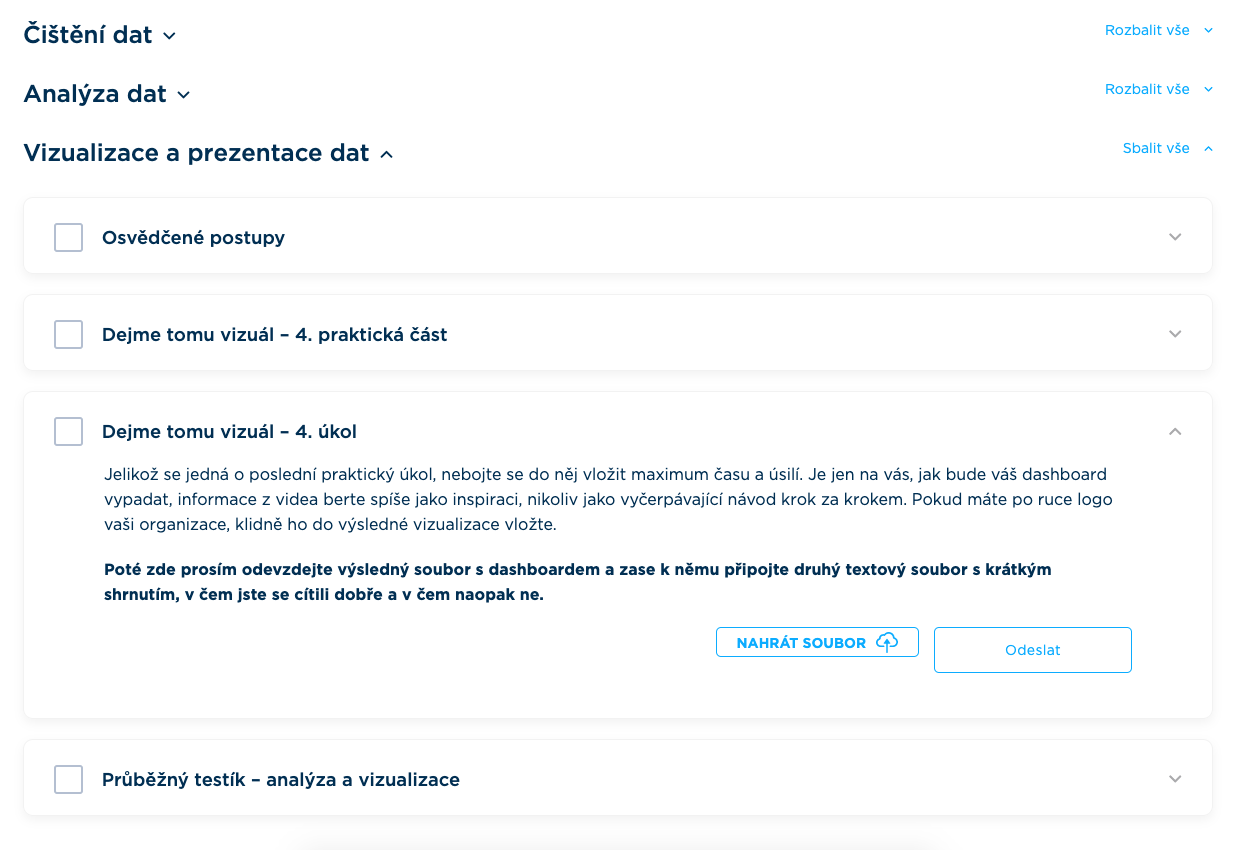
\includegraphics[width=1.1\textwidth]{digi-aktivity}  
    \caption{Závěrečná aktivita, která obsahuje zadání praktického úkolu}
    \label{digi-aktivity}
\end{figure}

Všechny aktivity lze dále kategorizovat podle svého typu, který determinuje, jaká edukační komponenta je v~dané aktivitě využita. Kromě typů \emph{nahrát soubor} a~\emph{test typeform} (viz níže) musí student po dokončení vybrané aktivity vždy zatrhnout políčko \emph{Označit aktivitu za splněnou}, které aktualizuje progres studenta a~přesměruje ho na následující aktivitu.

V~našem online kurzu využíváme výhradně těchto pět typů aktivit, které jsme pro účely tohoto e-learningu vytvořili na základě výsledků z~provedené přehledové studie online kurzů:

\begin{itemize}
\tightlist
\item
  \emph{přečíst text} -- student musí pro splnění tohoto typu aktivity přečíst textový materiál, který je typicky doplněn o~vizualizace, jež téma obsahově doplňují, případně jej graficky člení pro větší přehlednost;
\item
  \emph{zhlédnout video} -- v~těchto aktivitách musí student zhlédnout video, které nejčastěji vysvětluje danou problematiku prostřednictvím praktických ukázek;
\item
  \emph{vložit text} -- tyto aktivity rozšiřují první typ, tedy textový materiál doplňují o~textové pole, do nějž musí student zadat odpověď na otázku vztahující se k~tématu;
\item
  \emph{nahrát soubor} -- aktivity tohoto typu jsou umístěny za výukovými videy, protože v~rámci nich student odevzdává vlastní vypracovanou práci spolu s~krátkou textovou reflexí\footnote{Krátkou reflexi jsme po odevzdání praktických úkolů začlenili z~toho důvodu, aby měl student možnost zapřemýšlet nad nově nabytými dovednostmi a~případnými nejasnostmi, které mohou spojeny buď s~probíranou problematikou anebo s~formátem samotného kurzu.};
\item
  \emph{test typeform} -- v~těchto aktivitách student vypracovává krátký kvíz, jehož cílem je připomenout hlavní znalosti a~dovednosti, které si v~rámci minulých aktivit osvojil. Při špatné odpovědi kvíz studenta naviguje ke konkrétní aktivitě, která látku vysvětluje, student může posléze svoji odpověď změnit a~znovu odpovídat (viz Obrazek \ref{digi-kviz} a~\ref{digi-kviz-0}).
\end{itemize}

\begin{figure}[hb!]   
    \centering
    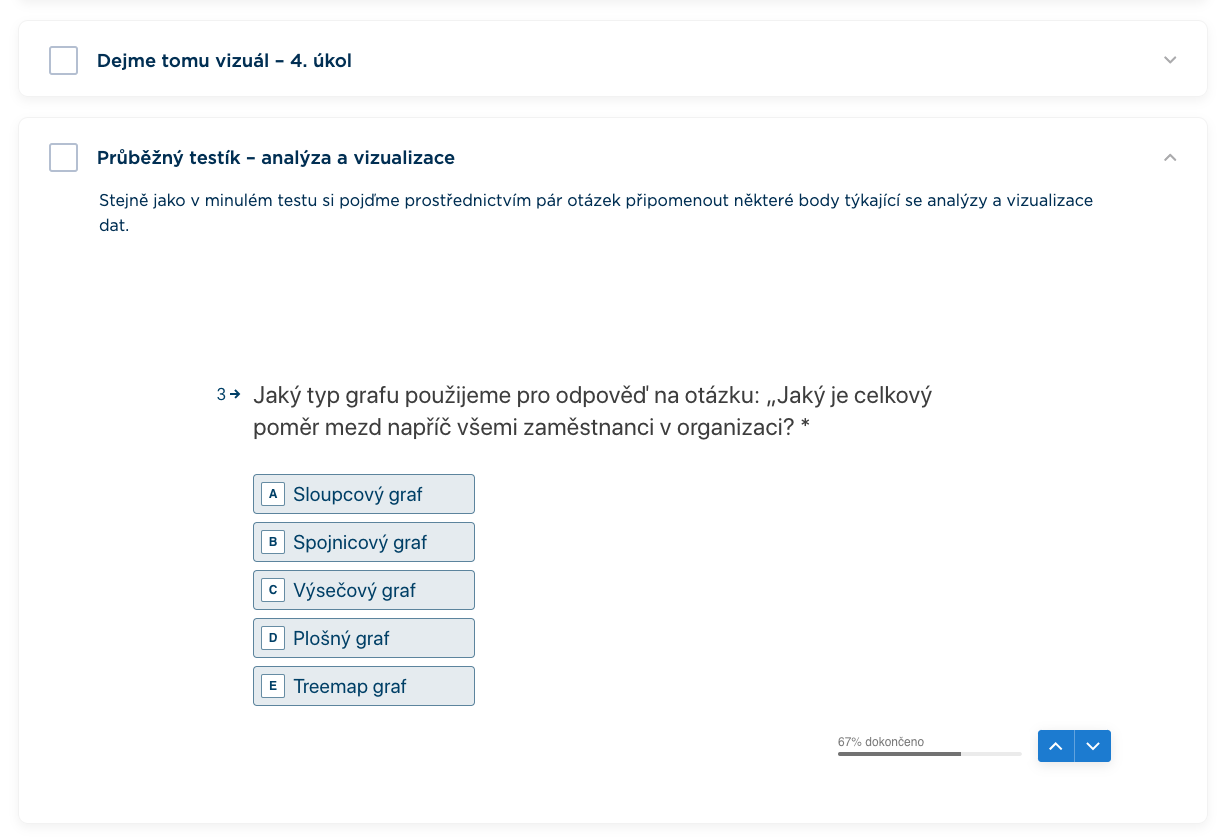
\includegraphics[width=\textwidth]{digi-kviz}  
    \caption{Příklad otázky z~průběžného kvízu týkající se tématu analýza a~vizualizace dat}
    \label{digi-kviz}
\end{figure}

\begin{figure}[hb!]   
    \centering
    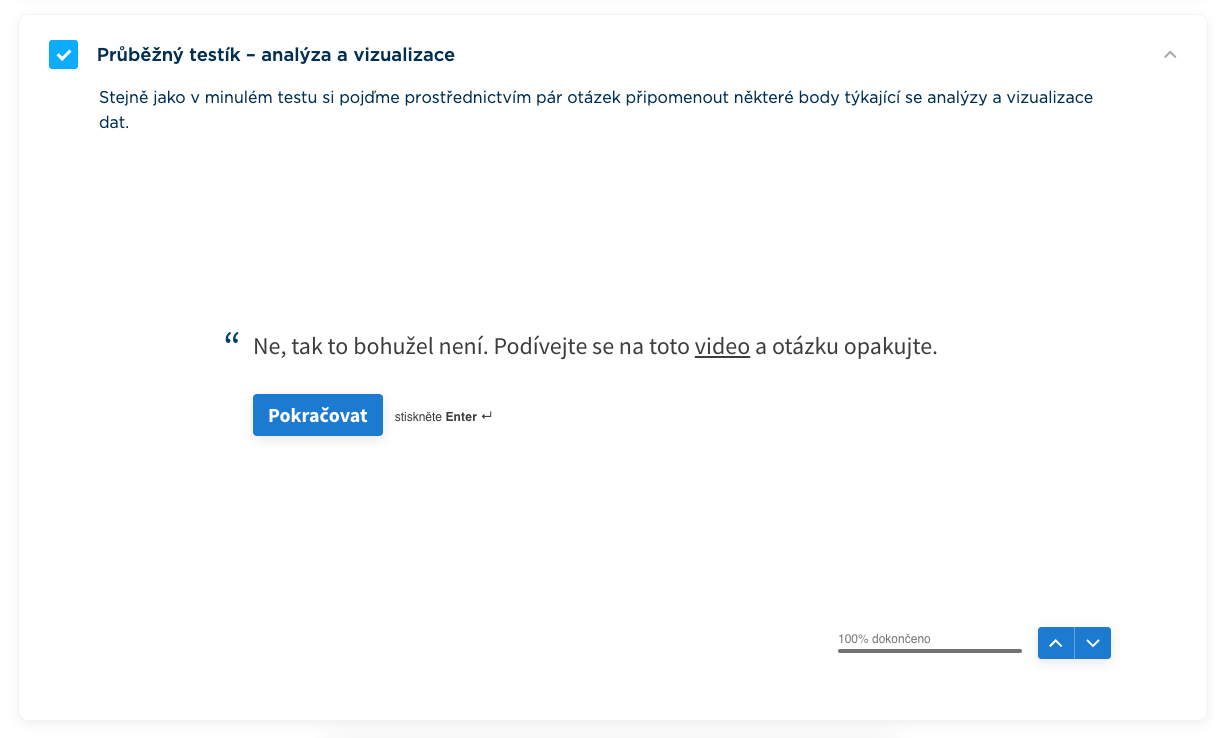
\includegraphics[width=\textwidth]{digi-kviz-0}  
    \caption{Příklad otázky z~průběžného kvízu týkající se tématu analýza a~vizualizace dat}
    \label{digi-kviz-0}
\end{figure}

Pro úspěšný průchod celým kurzem je zapotřebí mít splněné všechny dílčí aktivity včetně kvízů a~korektně odevzdané všechny praktické úkoly. Kurz byl navržen tak, aby byly všechny odevzdané úkoly zkontrolovány pověřenou osobou -- chceme tak docílit k~poskytnutí individuální zpětné vazby každému jednotlivému studentovi.

\hypertarget{moduly}{%
\section{Moduly}\label{moduly}}

V~poslední podkapitole popíšeme jednotlivé obsahové bloky (dále jen moduly), které dělíme podle toho, jaký vzdělávací cíl splňují, a~tedy zda spadají do teoreticky nebo prakticky zaměřené části kurzu\footnote{Prostřednictvím celkové stylizace kurzu směřujeme k~co největší popularizaci tématu, proto jsou některé názvy jednotlivých obsahových bloků a~aktivit pojaty méně formálním způsobem.}.

\begin{figure}[hb!]   
    \centering
    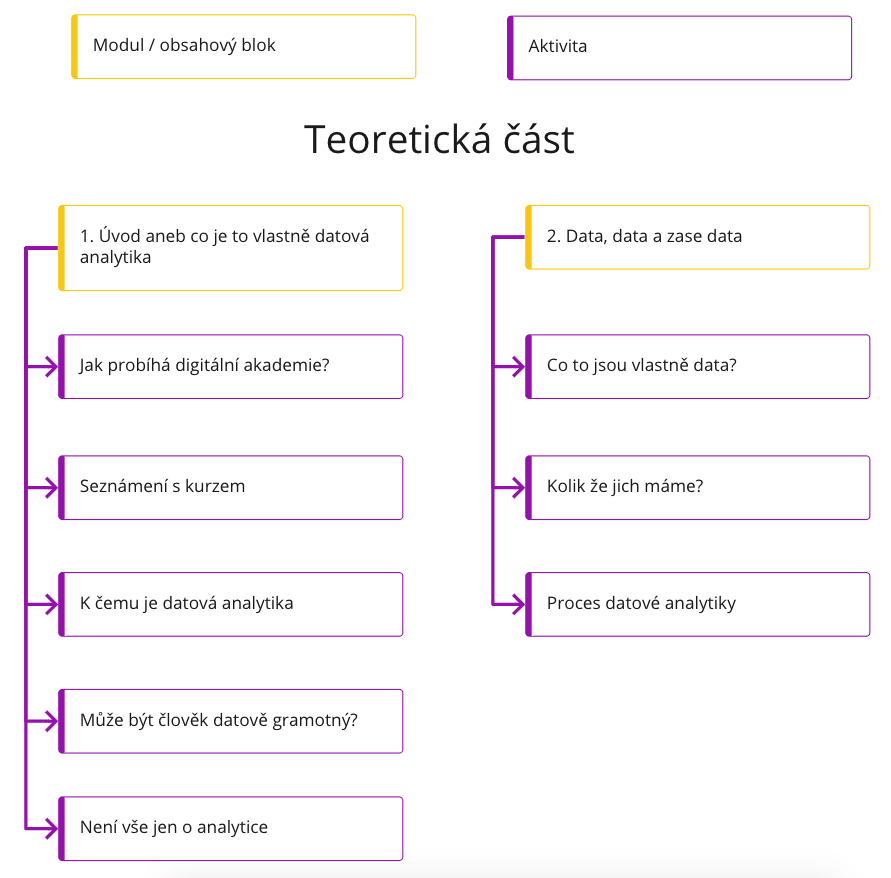
\includegraphics[width=\textwidth]{schema-1}  
    \caption{Schéma teoretické části}
    \label{schema-1}
\end{figure}

\begin{figure}[hb!]   
    \centering
    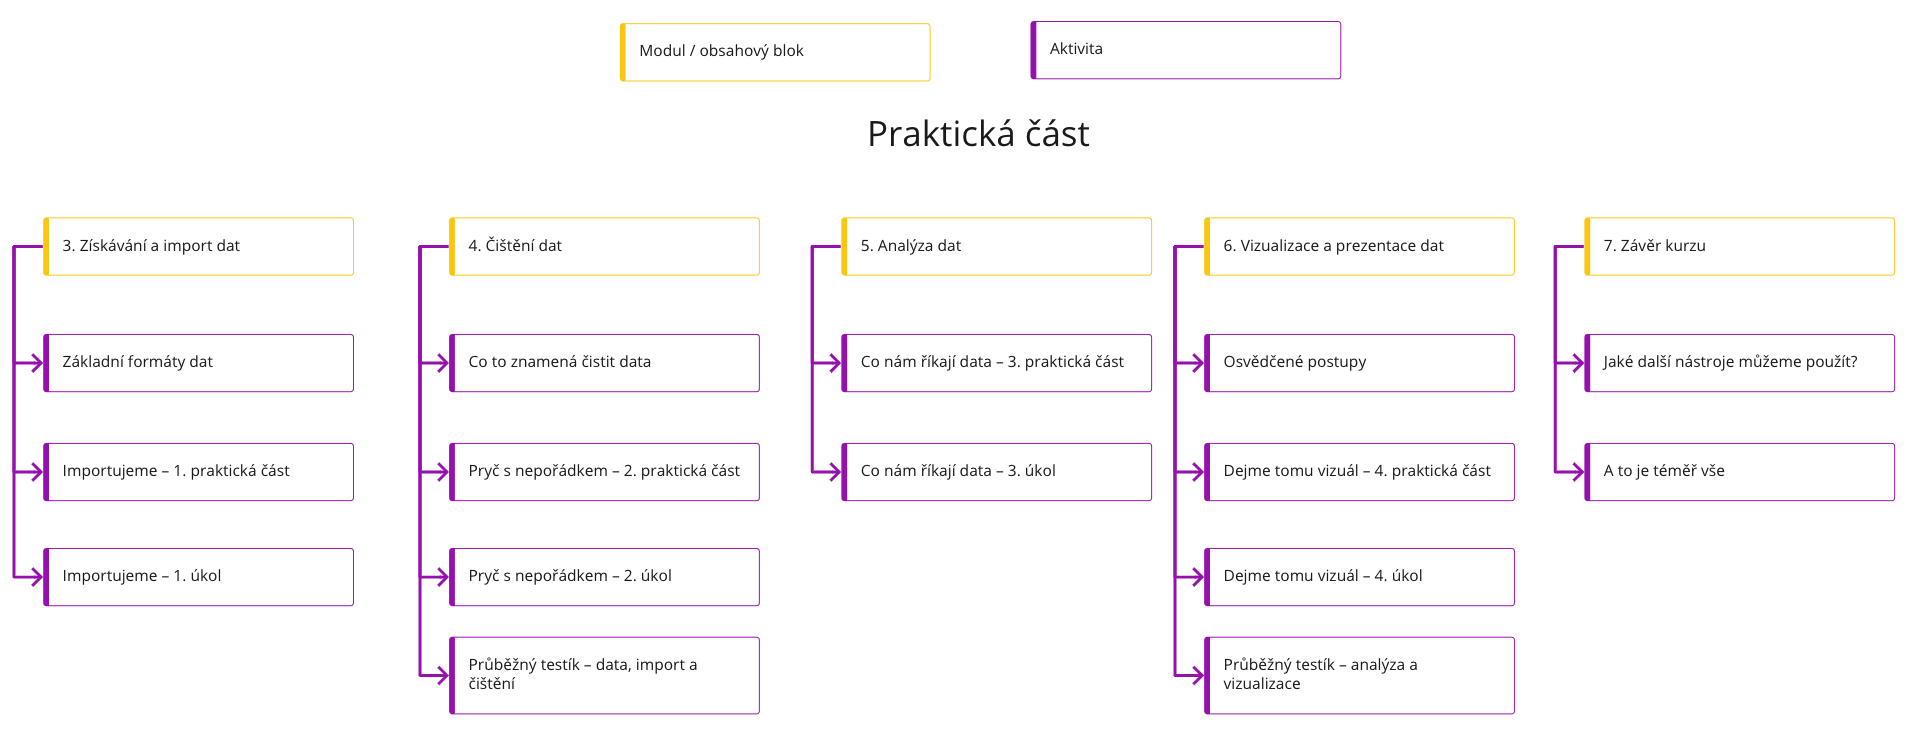
\includegraphics[width=\textwidth]{schema-2}  
    \caption{Schéma praktické části}
    \label{schema-2}
\end{figure}

\hypertarget{uxfavod-aneb-co-je-to-vlastnux11b-datovuxe1-analytika}{%
\subsection{Úvod aneb co je to vlastně datová analytika}\label{uxfavod-aneb-co-je-to-vlastnux11b-datovuxe1-analytika}}

První teoretický modul si klade za cíl uvést studenta do kontextu celého kurzu -- představuje mu možnosti online prostředí, vysvětluje, jak probíhá průchod kurzem, a~uvádí osnovu kurzu. Ještě před samotnou teorií týkající se úvodních témat datové analytiky je student seznámen se skutečností, že v~druhé, praktické části kurzu, bude sám participovat na svém vlastním řešení, prostřednictvím kterého by si měl vyzkoušet základní techniky datové analytiky.

V~dalších částech tohoto modulu je co srozumitelným způsobem vysvětleno, proč je důležité datovou analytiku v~organizacích využívat a~jakou přidanou hodnotu může mít při tvorbě firemních rozhodnutí. V~této části jsme se také zaměřili na koncept \emph{datově orientované organizace}, v~rámci kterého jsme se snažili vztáhnout téma datové gramotnosti právě na organizační prostředí a~znovu tak studenta motivovat ke studiu datové analytiky.

V~poslední aktivitě jsme se pak zmínili o~příbuzných pojmech, které se s~datovou analytikou pojí (např. \emph{Big Data} a~\emph{IoT}) a~jasně jsme vymezili příbuzené disciplíny jako jsou \emph{Data Science} a~\emph{Data Engineering}. Z~celkového hlediska tento modul naplňuje první dva vzdělávací cíle kurzu.

\hypertarget{data-data-a-zase-data}{%
\subsection{Data, data a~zase data}\label{data-data-a-zase-data}}

Druhý teoretický obsahový blok zpracovává problematiku spojenou s~definicí dat -- snaží se studentovi vysvětlit, co si lze pod pojmem data představit a~jakým způsobem můžeme data dělit a~kategorizovat podle daných potřeb. V~této sekci již studenta uvádíme do tématu prostřednictvím krátkého popularizačního videa a~následně pomocí stručného článku pobízíme k~zamyšlení, s~jakým typem dat student nejčastěji pracuje ve svém prostředí.

Na závěr modulu představujeme obsah praktické části kurzu, kterým je proces datové analytiky. Ve videu popisujeme jednotlivé fáze procesu a~snažíme se akcentovat fakt, že data nejsou totéž co informace, ale že ze surových dat informace získáváme právě prostřednictvím analýzy a~následné vizualizace. Tato část tak splňuje třetí a~částečně čtvrtý vzdělávací cíl kurzu.

\hypertarget{zuxedskuxe1vuxe1nuxed-a-import-dat}{%
\subsection{Získávání a~import dat}\label{zuxedskuxe1vuxe1nuxed-a-import-dat}}

V~tomto modulu je studentovi představen první krok datové analytiky, jenž se zabývá importem dat. Na začátku obsahového bloku je nejprve popsána problematika týkající se formátů dat. Popisujeme základní charakteristiky textových a~binárních souborů a~uvádíme základní příklady souborových přípon spolu s~jejich využitím. Na konci první aktivity rozlišujeme dva nejčastěji používané textové formáty pro uchovávání tabulkových dat s~příponami \emph{.csv} a~\emph{.tsv}, se kterými následně pracujeme v~praktické ukázce.

Hlavní částí tohoto modulu je demonstrační video, v~rámci kterého na konkrétním modelovém datasetu\footnote{Zjednodušený dataset obsahuje data vztahující se k~provedeným objednávkám fiktivní organizace. Každý záznam objednávky je tvořen těmito atributy: jméno prodejce, region, účet, částka, měsíc a~datum (atribut datum jsme zde přidali pro účely zpracování speciálního datového typu.)} z~fiktivního firemního prostředí představujeme možnosti importu dat. Ohledně výběru datasetu jsme se inspirovali přístupy z~analyzovaných online kurzů, nicméně jsme jej upravili tak, aby co nejvíce vyhovoval naší cílové skupině začátečníků.

Po zhlednutí výukového videa je student vyzván k~aplikaci nabytých dovedností na stejném datasetu, který jsme použili v~demonstraci. V~tomto úkolu ještě není po studujícím vyžadovaná žádná velká invence, jde primárně o~zadání, jehož cílem je otestovat studentovo prostředí a~vyzkoušet funkčnost webové \emph{odevzdávárny}.

Na konci tohoto modulu by tak mělo být studentovi zřejmé, že jednotlivé fáze datové analytiky na sebe navazují, a~je proto zapotřebí vypracovat daný úkol vždy korektním způsobem (tedy alespoň tak, jak je znázorněno v~daném demonstračním videu), protože se v~dalších praktických částech vychází vždy z~výsledků předešlého modulu. Tento obsahový blok naplňuje pátý vzdělávací cíl kurzu\textbackslash footnote\{S ohledem na skutečnost, že se všechny praktické moduly týkají procesu datové analytiky, naplňují vždy současně i~čtvrtý cíl kurzu).

\hypertarget{ux10diux161tux11bnuxed-dat}{%
\subsection{Čištění dat}\label{ux10diux161tux11bnuxed-dat}}

Obsahový blok zabývající se čištěním dat pokládáme za jeden z~nejdůležitějších, přestože se tohle téma v~jiných online kurzech neobjevuje příliš často. Vycházíme z~toho, že je na tomto kroku přímo závislá kvalita vlastní analýzy dat, protože se nepřesnosti ve vstupních datech lehce propisují do zkoumaných vztahů napříč daty. Tento fakt se snažíme studentovi představit v~úvodní aktivitě, která se prostřednictvím textového materiálu snaží poukázat na nejčastější chyby v~datech a~na způsoby jejich řešení.

V~další části v~demonstračním videu využíváme tyto znalosti k~opravení nejdůležitějších chyb v~našem modelovém datasetu. Výstupem z~této části by měla být očištěná tabulková data, která lze dále efektivně zpracovávat. V~tuto chvíli je již studentovi dán v~rámci praktického úkolu větší prostor, protože je pobídnut k~opravě většího množství chyb, než bylo vyřešeno v~ukázce. Taktéž zde pracujeme s~jednoduchou formou zpětné vazby, protože se zde studujícího ptáme na jeho subjektivní pohled týkající se obtížnosti problematiky.

Nakonec v~tomto modulu zavádíme první kvíz, který připomíná základní informace týkající se dat, jejich importu a~čištění. Tato celá část pracuje s~šestým cílem.

\hypertarget{analuxfdza-dat}{%
\subsection{Analýza dat}\label{analuxfdza-dat}}

Modul zpracovávající problematiku analýzy dat je klíčový z~hlediska tvorby nových informací z~očištěných dat. V~této částí studentovi téma rovnou představujeme pomocí výukového videa, v~rámci kterého ukazujeme, jakým způsobem lze zobrazovat vztahy napříč daty. Pro účely této ukázky využíváme nástroj kontingenční tabulky, který nám umožňuje vytvářet z~výchozího datasetu nové (kontingenční) tabulky a~na základě filtrů, numerických operací a~dalších metod pro analýzu dat zobrazovat vzájemné vztahy mezi daty. Tyto tabulky pak slouží jako zdroj dat pro grafy a~další vizualizace, protože obsahují právě ty informace, které jsou užitečné pro rozhodování založeném na datovém základě.

Student má v~tomto modulu za úkol provést vlastní analýzu dat, nemusí se ale přímo vázat na konkrétní příklady z~ukázky. Naopak je motivován k~hledání zajímavějších vztahů napříč daty a~k~experimentům nad funkcemi kontingenčních tabulek. Zároveň je od studenta znovu vyžadována zpětná vazba (která částečně plní funkci reflexe) na pocity, které se s~tvorbou analýzy pojily, a~případně na konkrétní části, kde se studující cítil frustrován. Celkově tento modul naplňuje sedmý vzdělávací cíl kurzu.

\hypertarget{vizualizace-a-prezentace-dat}{%
\subsection{Vizualizace a~prezentace dat}\label{vizualizace-a-prezentace-dat}}

Závěrečná část procesu datové analytiky se týká vizualizace a~prezentace dat. Tento modul je patrně nejrozsáhlejší, protože v~sobě obsahuje jak základní teorii k~tvorbě grafů, tak i~praktické cvičení vztahující se k~základním vizualizačním technikám. V~první aktivitě je student seznámen s~pojmem \emph{dashboard}\footnote{Zde jsme akcentovali otázku týkající se různorodosti příjemců informací. To znamená, že by si měl být student při prezentaci dat vždy vědom toho, jak zkušení uživatelé tento výstup přijímají, a~podle toho volit složitost daných vizualizací.} a~jsou zde představeny základní typy grafů spolu s~příklady otázek, na něž jednotlivé grafy typicky odpovídají.

Na tento teoretický text přímo navazuje poslední demonstrační video, které představuje základní principy a~možnosti vizualizace dat v~našem kontextu. Důraz se v~tomto případě klade i~na interaktivitu výsledné vizualizace, tedy aby bylo možné data v~rámci konečného \emph{dashboardu} částečně měnit na základě nově položené otázky. I~v~tomto posledním praktickém úkolu je student pobídnut k~tvorbě vlastního originálního řešení, předcházející video by mu mělo tak sloužit pouze jako inspirace a~základní osnova. A~stejně jako v~minulém modulu je od něj vyžadována zpětná vazba týkající se silných a~slabých stránek při tvorbě vizualizace. Tento předposlední obsahový modul splňuje osmí cíl kurzu.

\hypertarget{zuxe1vux11br-kurzu}{%
\subsection{Závěr kurzu}\label{zuxe1vux11br-kurzu}}

Poslední modul si klade za cíl celkově shrnout obsah kurzu a~nabídnout studentovi inspiraci pro případné navazující studium v~kontextu jiných analytických nástrojů. Druhou podstatnou částí je závěrečný kvíz, který se už netýká žádného z~témat spojených s~datovou analytikou, ale zaměřuje na získání zpětné vazby ke kurzu. Prostřednictvím odpovědí z~tohoto dotazníku můžeme dále případně modifikovat obsah, pozměnit formu úkolů, případně přidat další související témata. Tento poslední modul tak odpovídá poslednímu vzdělávacímu cíli.
